% !TeX root = index.tex
% define document class
\documentclass{scrreprt}

% set variables
\newcommand{\varAuthor}{Sami Hindi}
\newcommand{\varCandidate}{\textbf{\varAuthor} \\ sami.hindi@renuo.ch} % Kandidat/in
\newcommand{\varResponsibleSpecialist}{\textbf{Raphael Nestler} \\ raphael.nestler@renuo.ch} % verantwortliche Fachkraft
\newcommand{\varVocationalTrainer}{\textbf{Stephan Amstutz} \\ stephan.amstutz@ksh.ch} % Berufsbildner/in
\newcommand{\varPrimaryExpert}{\textbf{Umachandran Aschvin} \\ aschvin00@gmail.com} % Hauptexperte
\newcommand{\varSecondaryExpert}{\textbf{Kevin Cina} \\ pk19@cinas.ch} % Nebenexperte
\newcommand{\varCompany}{Renuo AG} % Firmenname
\newcommand{\varCompanyDepartment}{Entwicklung} % Abteilungsname
\newcommand{\varTitle}{Meine IPA}
\newcommand{\varVersion}{0.3} % Versionsnummer: Pro IPA-Tag um 0.1 erhöhen
\newcommand{\varExaminationBoard}{Prüfungskomission 19} % Prüfungsorganisation
\newcommand{\varExaminationBoardDepartment}{Informatik Applikationsentwicklung} % Fachrichtung

% apply ipa package
\usepackage{../lib/ipa}
\usepackage{../lib/tikz-uml}
\usepackage{url}
\usepackage{amssymb}
\usepackage{bbding}

\lohead[\varTitle]{\varTitle}
\lofoot[\today]{\today}
% see B6.5
\cfoot[\varAuthor\ / \varCompany\\Version \varVersion]{\varAuthor\ / \varCompany\\Version \varVersion}
\rofoot[Seite \pagemark{} von \pageref{LastPage}]{Seite \pagemark{} von \pageref{LastPage}}

% load sources
\addbibresource{sources.bib}

% make glossaries
\makenoidxglossaries

% define glossary entries
% see B6.6
\newglossaryentry{Organigramm}{
  name={Organigramm},
  description={Ein Organigramm stellt eine Organisation und deren Aufbauorganisation grafisch dar.}
}

% create document
\begin{document}

  % set page numbering
  \pagenumbering{roman}

  % set page style
  \pagestyle{scrheadings}

  % include title page
  \thispagestyle{empty}

  \begin{center}
  \makebox[\textwidth]{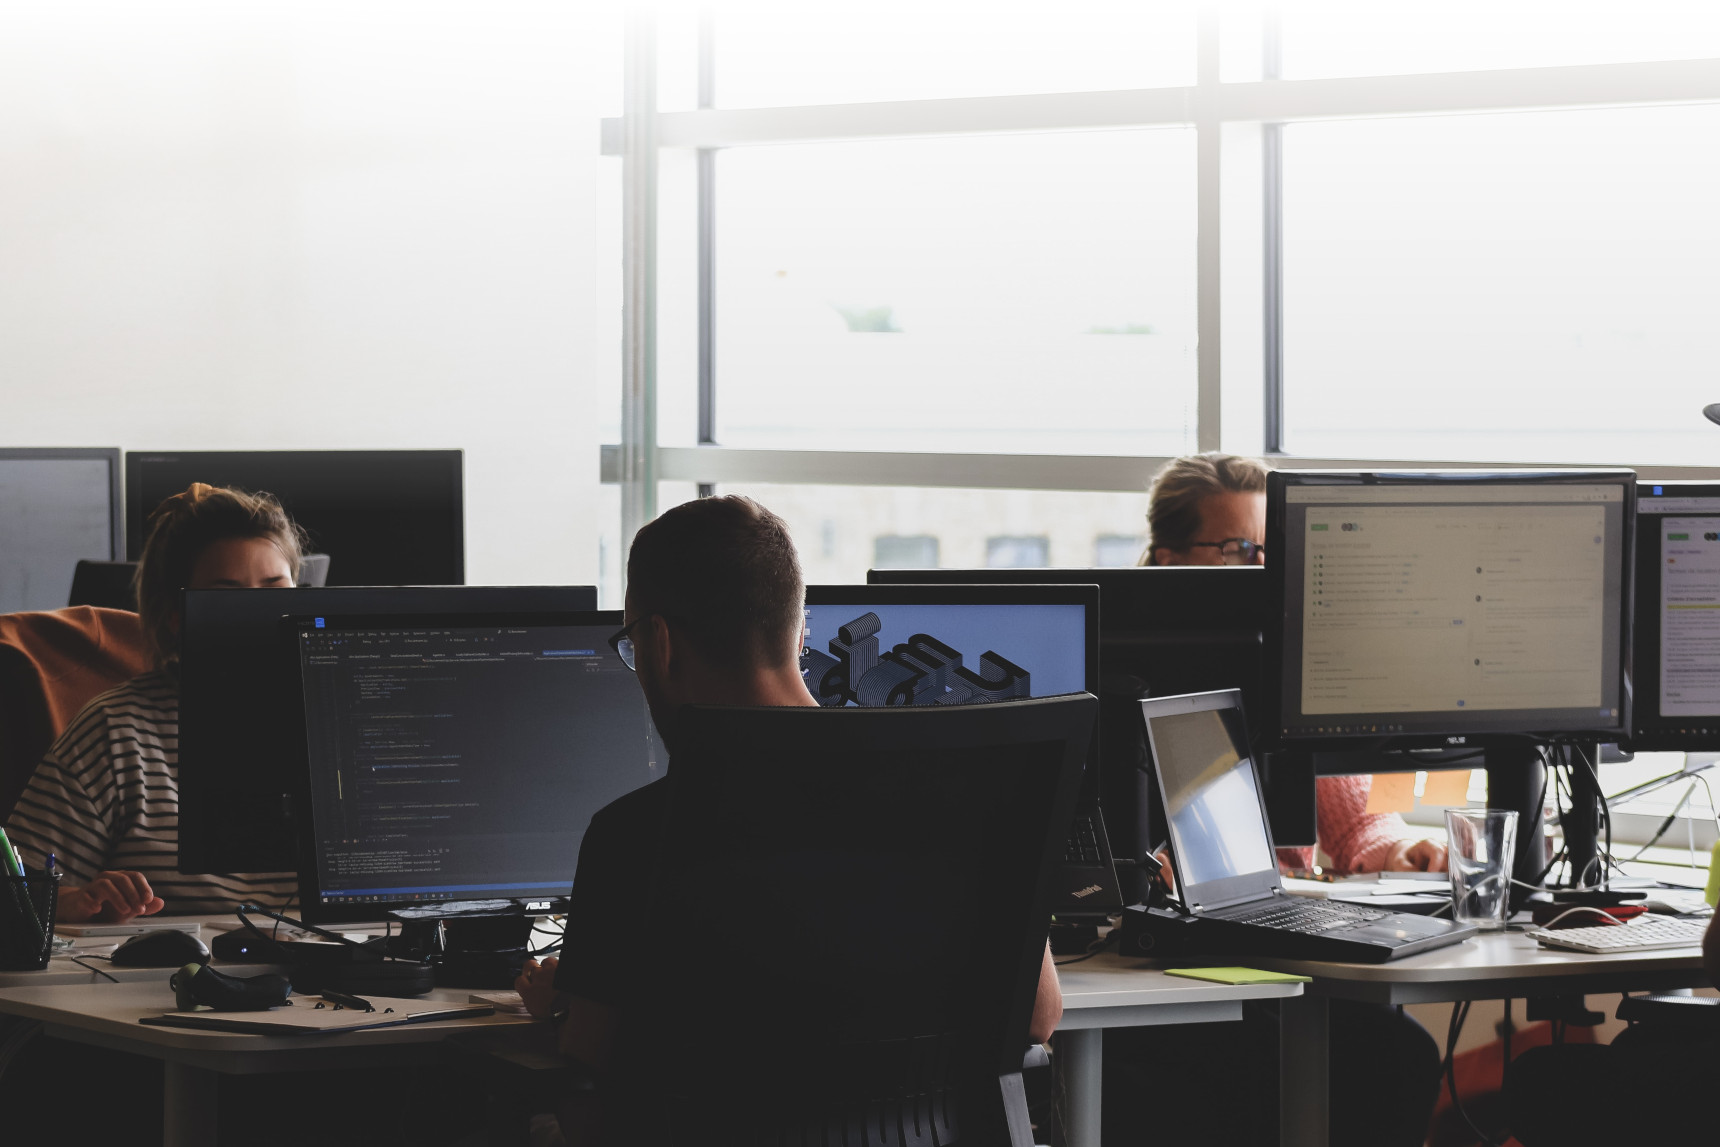
\includegraphics[width=1.1\paperwidth]{images/title.jpg}}
\end{center}
\vspace*{1cm}
{\fontsize{28}{28}\selectfont \varTitle}\\[0.25cm]
{\fontsize{16}{16}\selectfont \varAuthor}\\[0.25cm]
{\fontsize{16}{16}\selectfont \varCompany}

  \newpage
  \TileWallPaper{\paperwidth}{\paperheight}{images/background.pdf}

  % see A1.3
  % see B6.3
  % generate the table of contents
  \tableofcontents

  % finish page
  \clearpage

  % use the arabic numbering system
  \pagenumbering{arabic}

  % reset page counter
  \setcounter{page}{1}

  % see B6.1a
  % create a phantom toc entry for "Umfeld und Ablauf"
  \clearpage\phantomsection\addcontentsline{toc}{part}{Umfeld und Ablauf}

  % [2]: Seite 11
\chapter{Aufgabenstellung}

In diesem Kapitel findest du die vollständige Aufgabenstellung im originalen Wortlaut.

\section{Ausgangslage}

Die Renuo AG ist eine Software-Agentur, die sich auf die Entwicklung von Webanwendungen mit Ruby on Rails spezialisiert hat. Bei der Renuo AG nutzen wir eine Software namens \textbf{Redmine} zur Projektverwaltung. Redmine bietet auch Funktionen zur Verwaltung von Issues (Aufgaben oder Fehlerberichte), allerdings gestaltet sich die Suche nach bestimmten Issues oft schwierig, wenn man nicht genau weiss, wonach man suchen sollte.

\begin{figure}[h]
    \centering
    
\includegraphics[width=0.5\textwidth]{images/redmine.png}
    \caption{Redmine Logo}
    \label{fig:redmine}
\end{figure}

Da Redmine eine Open-Source-Software ist, ist der Source-Code öffentlich verfügbar. Das ermöglicht es nicht nur, die Funktionsweise von Redmine nachzuvollziehen, sondern auch, die Funktionalität durch eigene oder bereits existierende Plugins zu erweitern.

Einige der Funktionen, die Redmine \textquotedblleft out-of-the-box\textquotedblright\ mitbringt, reichen für die Anforderungen der Renuo nicht immer aus. Ein Beispiel dafür ist die Suche nach Issues.

\begin{figure}[h]
    \centering
    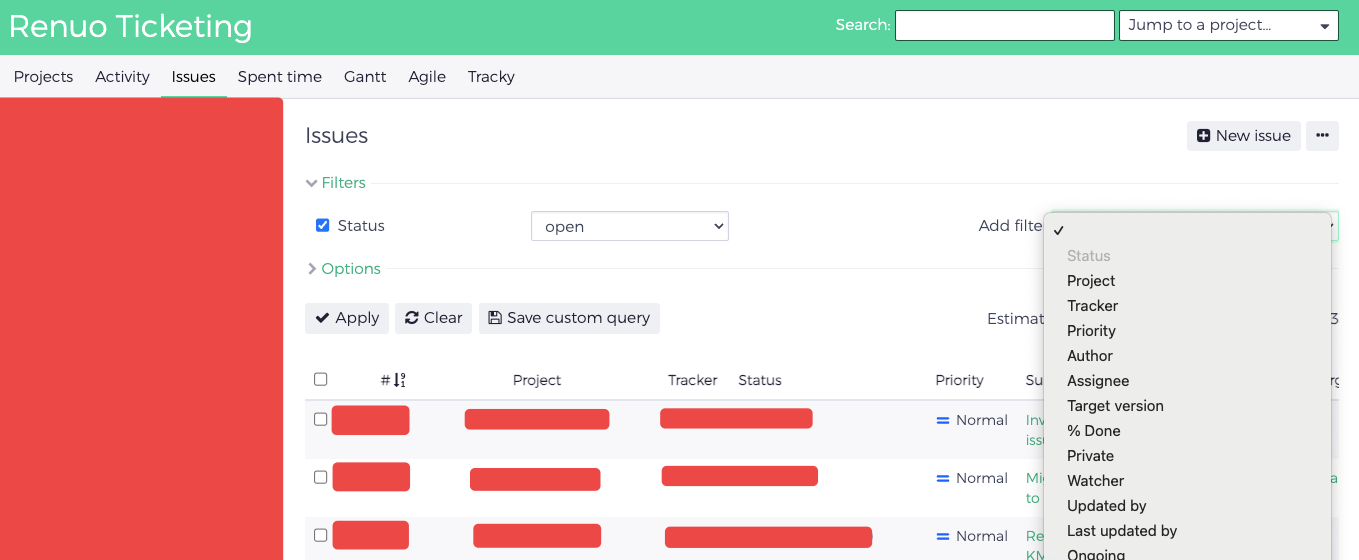
\includegraphics[width=1\textwidth]{images/redmine-search.png}
    \caption{Screenshot der Redmine Suchfunktion}
    \label{fig:redmine-search}
\end{figure}

Dieses Problem soll im Rahmen dieser IPA-Arbeit gelöst werden.

\section{Detaillierte Aufgabenstellung}

Das Ziel dieses Projekts ist es, die grundsätzliche Machbarkeit eines Ansatzes zur Verbesserung der Suche zu untersuchen. Dafür werden Informationen zu folgenden Punkten benötigt:

\begin{itemize}
    \item Qualität der neuen Suchergebnisse
    \item Performance der Suche
    \item Kosten
\end{itemize}

Die Software richtet sich an folgende Benutzerrollen:

\begin{itemize}
    \item \textbf{Admin:} Konfiguriert und verwaltet die Redmine-Installation und hat Zugriff auf einen Admin-Account.
    \item \textbf{User:} Sucht nach Tickets mit ähnlichen Inhalten und hat Zugriff auf einen normalen User-Account.
    \item Die Unterscheidung der Rollen erfolgt über das bestehende Rollensystem von Redmine (Admin-Flag in der Datenbank).
\end{itemize}

\subsection{Abkürzungen / Begriffe}

\begin{itemize}
    \item \textbf{Source-Code:} Der Quellcode eines Projekts
    \item \textbf{Embedding:} Ein Vektor, der einen Text oder einen Satz repräsentiert.
    \item \textbf{AI:} Artificial Intelligence, Künstliche Intelligenz
    \item \textbf{OpenAI:} Die Firma hinter \url{https://openai.com/}
    \item \textbf{OpenAI-API:} Schnittstellen von OpenAI \url{https://openai.com/api/}
    \item \textbf{ERB:} Embedded Ruby. Templating Engine für Ruby (\url{https://rubyapi.org/o/erb})
    \item \textbf{Slim:} Template Engine für Ruby (\url{https://slim-template.github.io/})
    \item \textbf{CI:} Continuous Integration
    \item \textbf{SaaS:} Software-as-a-Service
\end{itemize}

\subsection{Folgende User-Stories sollen umgesetzt werden:}

\begin{itemize}
    \item \textbf{F1:} Als Admin kann ich das AI-Search-Redmine-Plugin herunterladen und installieren. Die Anweisungen im README des GitHub-Repositories reichen für die Installation aus. Das Plugin ist nach der Installation nicht automatisch aktiviert.
    \item \textbf{F2:} Als Admin kann ich die für das Plugin benötigten Zugangsdaten als Umgebungsvariablen hinterlegen (OpenAI-API-Key).
    \item \textbf{F3:} Als User kann ich nach Tickets suchen, wobei die Ergebnisse wie bei der bestehenden Suche angezeigt werden. Es ist vom Lernenden selbst zu entscheiden, welche Ticket-Felder, Kommentare und Zeiteintrag-Kommentare in das Embedding einfliessen. Dabei sollen die Relevanz der Felder für die Suchergebnisse, die Häufigkeit der Regenerierung der Embeddings bei Datenänderungen und der Entwicklungsaufwand berücksichtigt werden. Ebenso ist zu bestimmen, welches AI-Modell von OpenAI verwendet wird. Dabei sollen Eignung, Kosten und Performance evaluiert werden. Es genügt, sich auf die Empfehlungen und Dokumentation von OpenAI zu stützen; ein direkter Vergleich im Betrieb ist nicht erforderlich.
    \item \textbf{F4:} Die Suche steht nur Usern mit einer entsprechenden Entwickler- oder Managerrolle zur Verfügung.
    \item \textbf{F5:} Die Suchergebnisse dürfen nur Tickets enthalten, auf die der User auch tatsächlich Zugriff hat.
\end{itemize}

Es gelten folgende nicht-funktionalen Anforderungen:

\begin{itemize}
    \item \textbf{Software-Design:} Das Plugin muss so weit wie möglich von Redmine entkoppelt sein. Beispielsweise sollen bestehende Redmine-Tabellen nicht verändert werden (stattdessen Join-Tabellen verwenden).
    \item \textbf{Software-Design:} Das Plugin soll sich an die Coding-Guidelines von Redmine halten und bereits vorhandene Bibliotheken nutzen (z.B. Minitest, ERB statt Slim).
    \item \textbf{Software-Design:} Die Generierung der Embeddings soll im Hintergrund erfolgen.
    \item \textbf{Software-Design:} Die Anbindung der OpenAI-API soll so gestaltet sein, dass ein Wechsel des AI-Modells einfach möglich ist – insbesondere mit Blick darauf, später ein lokales AI-Modell einsetzen zu können.
    \item \textbf{Maintainability:} Das Plugin soll die Vanilla-Redmine-Versionen 5.1.x und 6.0.x unterstützen. Die speziell angepasste Redmine-Variante von Renuo muss nicht berücksichtigt werden.
    \item \textbf{Dokumentation:} Die Funktionsweise des Plugins muss im README des Projekts kurz beschrieben werden.
    \item \textbf{Tests:} Der Happy Path muss durch automatisierte End-to-End-Tests (System-Tests) abgedeckt sein.
    \item \textbf{Tests:} Die Unit-Test-Abdeckung des Plugins beträgt 100\%.
    \item \textbf{Tests:} Zugriffe auf die OpenAI-API müssen in den automatisierten Tests gemockt werden.
\end{itemize}

\subsection{Testumgebung}

Für die automatisierten Tests soll GitHub Actions mit Ubuntu 24.04 verwendet werden. Postgres wird dabei als Service eingebunden. Getestet wird mit Redmine 5.1 und 6.0. Die System-Tests werden mit der auf GitHub Actions verfügbaren Chrome-Version im "Headless"-Modus durchgeführt (siehe \url{https://github.com/actions/runner-images/blob/main/images/ubuntu/Ubuntu2404-Readme.md}).

Für manuelle Tests und Demonstrationen wird das MacBook des Kandidaten verwendet, das nach dem \textquotedblleft Renuo Laptop Setup Guide\textquotedblright\ eingerichtet ist.

\section{Mittel und Methoden}

Für die IPA werden folgende Technologien eingesetzt:

\begin{itemize}
    \item Redmine 5.1 und 6.0 (Plugin-Kompatibilität)
    \item Ruby on Rails 6.1 und 7.2 (Plugin-Kompatibilität)
    \item Ruby (3.2.8, da kompatibel mit Redmine 5.1 und 6.0)
    \item MiniTest (5.25.5 oder neuer)
    \item Rubocop (Version, die Redmine 6.0 verwendet: 1.68.0)
    \item HTML5 (HTML, JS, CSS)
    \item PostgreSQL (Version 16)
    \item pgvector (v0.8.0)
    \item GitHub / GitHub Actions (SaaS)
    \item OpenAI API (SaaS)
\end{itemize}

Wo relevant, wird die Software in englischer Sprache verwendet.

Die zu entwickelnde Software läuft auf dem MacBook des Kandidaten mit einer aktuellen Chrome-Version (Version 134 oder neuer). Das Laptop ist gemäss dem \textquotedblleft Renuo Laptop Setup Guide\textquotedblright\ eingerichtet.

Die Wahl der Software zur Dokumentation ist dem Kandidaten überlassen. In der Vergangenheit hat sich LaTeX mit \url{https://github.com/swissictedu/ipa-template} als Basis bewährt.

%\lipsum[10] % This line was commented out or removed in the previous step

  % [2]: Seite 11
\chapter{Deklaration}

Folgender Abschnitt beschreibt die Vorkenntnisse des Kandidaten und dessen Vorbereitung.

\section{Vorkenntnisse}

Der Lernende hat seit dem Praktikumsbeginn (1. August 2024) mit Ruby on Rails gearbeitet. Auch wurden die Tests in dieser Zeit mit RSpec und Capybara geschrieben und die Code-Qualität mit Rubocop überprüft. Ebenfalls seit dem Praktikumsstart wurde Git zusammen mit Github eingesetzt. Code-Reviews gehören ebenfalls zur täglichen Arbeit (sowohl Code Reviews durchführen wie auch entgegennehmen). SemaphoreCI wird ebenfalls seit Praktikumsbeginn eingesetzt.

\section{Vorarbeiten}

Folgende Arbeiten müssen vorab erledigt werden:

\begin{itemize}
  \item[\checkmark] Boilerplate Redmine-Plugin wird lokal so aufgesetzt, dass gegen Vanilla-Redmine 5.1.x, 6.0.x mit Postgres getestet werden kann. (Bis 18.4. abgeschlossen)
  \item[\checkmark] GitHub-Repository wird erstellt (Bis 25.4 abgeschlossen)
  \item[\checkmark] Erstellen des OpenAI API Tokens. (Bis 25.4. abgeschlossen)
  \item[\checkmark] Einlesen in die [Redmine-Plugin-Dokumentation](https://www.redmine.org/boards/4/topics/45309): (Bis 2.5. abgeschlossen)
  \item[\checkmark] Einlesen in Vector Search und Embeddings (Bereits abgeschlossen)
  \item[\checkmark] Lesen des [MiniTest-README](https://github.com/minitest/minitest) (Bis 2.5. abgeschlossen)
  \item[\checkmark] Einarbeitung in Software zur Erstellung der Dokumentation (Bis 8.5. abgeschlossen)
\end{itemize}

\section{Neue Lerninhalte}

\lipsum[13]

\section{Arbeiten in den letzten 6 Monaten}

\lipsum[14]

  % see B6.2a
\chapter{Projektaufbauorganisation}

% Diesen Abschnitt anpassen.
Das Projekt \placeholder\ wird in der Abteilung \enquote{\varCompanyDepartment} umgesetzt. Projektleiter ist \placeholder\ und für die IPA auch die verantwortliche Fachkraft. Für die fachliche Umsetzung des hier beschriebenen Projekts ist ausschliesslich die Zusammenarbeit zwischen \placeholder\ und dem Kandidaten notwendig.

Im Unterschied zur üblichen Arbeit im Betrieb, werden zwei Experten die Arbeit des Kandidaten begleiten und bewerten. Die Projektaufbauorganisation ist in \ref{fig:organigram} visualisiert.

\begin{figure}[H]
  \begin{multicols}{2}
    \begin{forest}
      for tree={draw,grow'=0,folder,align=left}
      [\textbf{\varCompany}
        [\textbf{HR}
          [(BB) \\ \varVocationalTrainer]
        ]
        [...]
        [\textbf{\varCompanyDepartment}
          [(VF) \\ \varResponsibleSpecialist]
          [(K) \\ \varCandidate]
        ]
      ]
    \end{forest}

    \begin{forest}
      for tree={draw,grow'=0,folder,align=left}
      [\textbf{\varExaminationBoard}
        [\textbf{\varExaminationBoardDepartment}
          [(HEX) \\ \varPrimaryExpert]
          [(NEX) \\ \varSecondaryExpert]
        ]
      ]
    \end{forest}
  \end{multicols}
  \caption[\enquote{Organigramm der am Projekt teilnehmenden Personen} visualisiert mit TikZ Forest]{\gls{Organigramm} der am Projekt teilnehmenden Personen}
  \label{fig:organigram}
\end{figure}
  % see A1.2
% see A3
% see B6.2b
\begin{landscape}
  \chapter{Zeitplan}
  Der Zeitplan basiert auf der Vorlage \cite{Buhler_ipa-timetable_2022} und zeigt mit einer Auflösung von zwei Stundenblöcken die geplanten und getätigten Aufwände.
  \begin{figure}[H]
    \begin{center}
      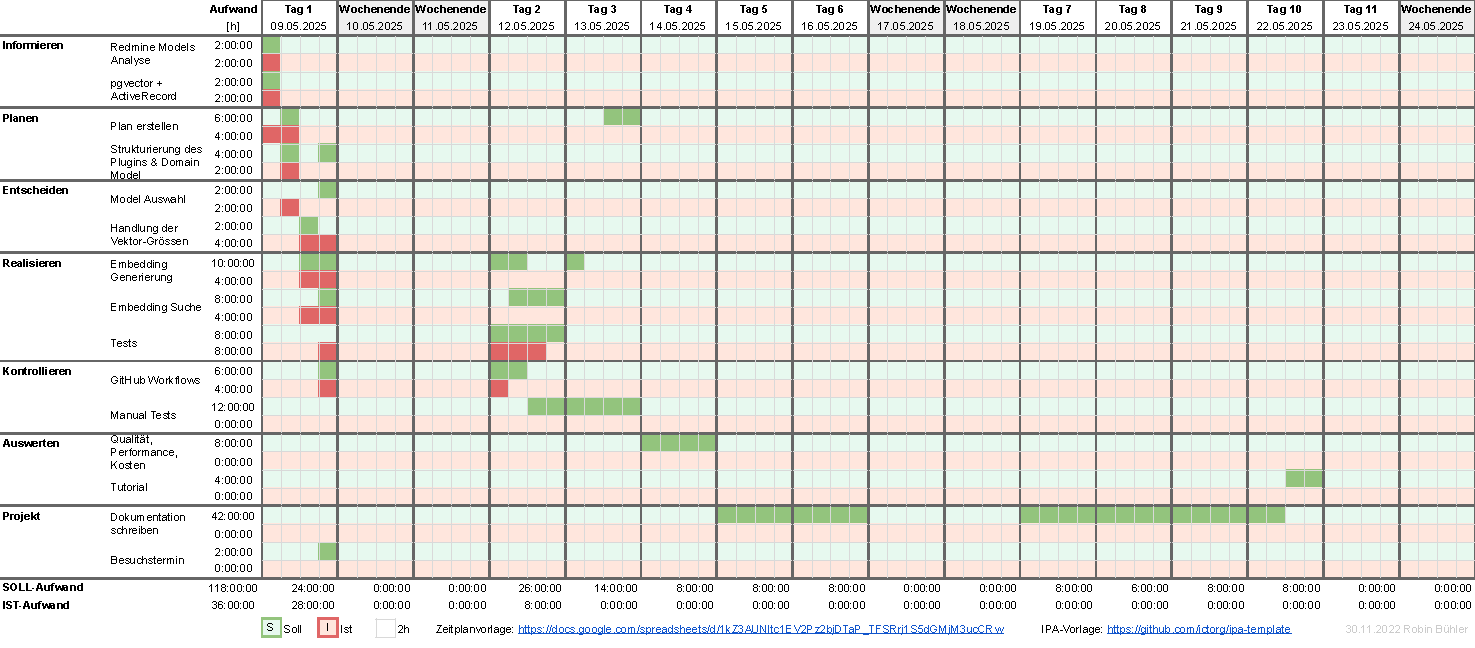
\includegraphics[width=1.55\textheight]{../res/timeplan.pdf}
    \end{center}
    \caption[\enquote{Zeitplan} erstellt mit Google Sheets]{Zeitplan}
    \label{fig:timeplan}
  \end{figure}
\end{landscape}

  % see A2.1
% see B6.2c
\chapter{Arbeitsjournal}

\section{Tag 1}
\begin{tabularx}{\textwidth}[H]{|c|X|}
  \hline
  Erledigte Arbeiten & Hier kann ich einfach was reinschreiben \\ \hline
  Ungeplante Arbeiten & \lipsum[24] \\ \hline
  Erfolge & \lipsum[25] \\ \hline
  Misserfolge & \lipsum[26] \\ \hline
  Hilfestellungen & \lipsum[27] \\
  \hline
\end{tabularx}

\newpage

\section{Tag 2}
\begin{tabularx}{\textwidth}[H]{|c|X|}
  \hline
  Erledigte Arbeiten & \lipsum[23] \\ \hline
  Ungeplante Arbeiten & \lipsum[24] \\ \hline
  Erfolge & \lipsum[25] \\ \hline
  Misserfolge & \lipsum[26] \\ \hline
  Hilfestellungen & \lipsum[27] \\
  \hline
\end{tabularx}

\newpage

\section{Tag 3}
\begin{tabularx}{\textwidth}[H]{|c|X|}
  \hline
  Erledigte Arbeiten & \lipsum[23] \\ \hline
  Ungeplante Arbeiten & \lipsum[24] \\ \hline
  Erfolge & \lipsum[25] \\ \hline
  Misserfolge & \lipsum[26] \\ \hline
  Hilfestellungen & \lipsum[27] \\
  \hline
\end{tabularx}

\newpage

\section{Tag 4}
\begin{tabularx}{\textwidth}[H]{|c|X|}
  \hline
  Erledigte Arbeiten & \lipsum[23] \\ \hline
  Ungeplante Arbeiten & \lipsum[24] \\ \hline
  Erfolge & \lipsum[25] \\ \hline
  Misserfolge & \lipsum[26] \\ \hline
  Hilfestellungen & \lipsum[27] \\
  \hline
\end{tabularx}

\newpage

\section{Tag 5}
\begin{tabularx}{\textwidth}[H]{|c|X|}
  \hline
  Erledigte Arbeiten & \lipsum[23] \\ \hline
  Ungeplante Arbeiten & \lipsum[24] \\ \hline
  Erfolge & \lipsum[25] \\ \hline
  Misserfolge & \lipsum[26] \\ \hline
  Hilfestellungen & \lipsum[27] \\
  \hline
\end{tabularx}

\newpage

\section{Tag 6}
\begin{tabularx}{\textwidth}[H]{|c|X|}
  \hline
  Erledigte Arbeiten & \lipsum[23] \\ \hline
  Ungeplante Arbeiten & \lipsum[24] \\ \hline
  Erfolge & \lipsum[25] \\ \hline
  Misserfolge & \lipsum[26] \\ \hline
  Hilfestellungen & \lipsum[27] \\
  \hline
\end{tabularx}

\newpage

\section{Tag 7}
\begin{tabularx}{\textwidth}[H]{|c|X|}
  \hline
  Erledigte Arbeiten & \lipsum[23] \\ \hline
  Ungeplante Arbeiten & \lipsum[24] \\ \hline
  Erfolge & \lipsum[25] \\ \hline
  Misserfolge & \lipsum[26] \\ \hline
  Hilfestellungen & \lipsum[27] \\
  \hline
\end{tabularx}

\newpage

\section{Tag 8}
\begin{tabularx}{\textwidth}[H]{|c|X|}
  \hline
  Erledigte Arbeiten & \lipsum[23] \\ \hline
  Ungeplante Arbeiten & \lipsum[24] \\ \hline
  Erfolge & \lipsum[25] \\ \hline
  Misserfolge & \lipsum[26] \\ \hline
  Hilfestellungen & \lipsum[27] \\
  \hline
\end{tabularx}

\newpage

\section{Tag 9}
\begin{tabularx}{\textwidth}[H]{|c|X|}
  \hline
  Erledigte Arbeiten & \lipsum[23] \\ \hline
  Ungeplante Arbeiten & \lipsum[24] \\ \hline
  Erfolge & \lipsum[25] \\ \hline
  Misserfolge & \lipsum[26] \\ \hline
  Hilfestellungen & \lipsum[27] \\
  \hline
\end{tabularx}

\newpage

\section{Tag 10}
\begin{tabularx}{\textwidth}[H]{|c|X|}
  \hline
  Erledigte Arbeiten & \lipsum[23] \\ \hline
  Ungeplante Arbeiten & \lipsum[24] \\ \hline
  Erfolge & \lipsum[25] \\ \hline
  Misserfolge & \lipsum[26] \\ \hline
  Hilfestellungen & \lipsum[27] \\
  \hline
\end{tabularx}


  % see B6.1a
  % create a phantom toc entry for "Projekt"
  \clearpage\phantomsection\addcontentsline{toc}{part}{Projekt}

  % See B1
\chapter{Kurzfassung}

Die Kurzfassung gibt einen Überblick über das vorliegende Projekt.

\section{Ausgangssituation}

\lipsum[20]

\section{Umsetzung}

\lipsum[21-22]

\section{Ergebnis}

\lipsum[22]
  % see A1.1a
\chapter{Informieren}

Die nachfolgende Dokumentation baut auf der Vorlage \cite{Buhler_ipa-template_2022} auf.

\section{Projektmanagement}

Das Projekt wird nach der Projektmanagementmethode IPERKA abgewickelt. Diese Methode passt zum Auftrag, weil der Auftrag in einer Iteration innerhalb von 10 Tagen wasserfallartig realisiert werden soll.

\subsection{Arbeitspakete}

Der Auftrag kann in folgende Arbeitspakete aufgeteilt und nach den Phasen der Projektmanagementmethode gegliedert werden:

\begin{itemize}
    \item Informieren
    \begin{description}
        \item[AP1: Anforderungen analysieren] Der Auftrag wird analysiert und daraus einzelne Arbeitspakete abgeleitet.
        \item[AP2: Lorem] \lipsum[2][1]
    \end{description}
    \item Planen
    \begin{description}
        \item[AP3: Lorem] \lipsum[2][2]
        \item[AP4: Lorem] \lipsum[2][3]
    \end{description}
    \item Entscheiden
    \begin{description}
        \item[AP5: Lorem] \lipsum[2][4]
        \item[AP6: Lorem] \lipsum[2][5]
    \end{description}
    \item Realisieren
    \begin{description}
        \item[AP7: Lorem] \lipsum[2][6]
        \item[AP8: Lorem] \lipsum[2][7]
    \end{description}
    \item Kontrollieren
    \begin{description}
        \item[AP9: Lorem] \lipsum[2][8]
        \item[AP10: Lorem] \lipsum[2][9]
    \end{description}
    \item Auswerten
    \begin{description}
        \item[AP11: Lorem] \lipsum[2][10]
        \item[AP12: Lorem] \lipsum[2][11]
    \end{description}
\end{itemize}

\section{Systemaufbau}
Im Folgenden wird die Einbettung des Systems in das Gesamtsystem gezeigt, sowie die vorhandenen Schnittstellen und Akteure beschrieben.

\subsection{Gesamtsystem}

\subsection{Schnittstellen}

\subsection{Akteure}

  % see A1.4
\chapter{Planen}

Die Zeitplanung wird in der Abbildung \ref{fig:timeplan} oberhalb gezeigt. Die restlichen Aspekte der Planung sind in diesem Kapitel dokumentiert.

\begin{figure}[H]
  \begin{center}
    \begin{tikzpicture}
      \begin{umlsystem}[x=0, y=0]{PkOrg}
      \end{umlsystem}
      \umlactor[x=-5, y=.1]{Verantwortliche Fachperson}
      \umlactor[x=5, y=.1]{Hauptexperte}
      \umlassoc{Verantwortliche Fachperson}{PkOrg}
      \umlassoc{Hauptexperte}{PkOrg}
    \end{tikzpicture}
  \end{center}
  \caption[\enquote{Systemkontextdiagramm} erstellt mit Tikz UML]{Systemkontextdiagramm}
  \label{fig:systemcontext}
\end{figure}

\section{Anwendungsfälle}

\section{Testkonzept}
Das Testkonzept beschreibt, wie und mit welchen Werkzeugen das Resultat auf seine Richtigkeit kontrolliert wird.

\subsection{Testmethoden}

\subsection{Testmittel}
  \chapter{Entscheiden}
  \chapter{Realisieren}

Verschiedene vorkonfigurierte Pakete helfen den Bericht, speziell die Realisierung, ansprechend zu formatieren und gestalten:

Aufruf von einer Aktion über ein Menü:
\menu{Extras > Settings > Rulers} \\
Drücken von Tastenkombinationen:
\keys{CTRL + R} \\
Verzeichnispfade:
\directory{C:/Windows/system32/hosts.txt} \\
Quellcode:

\begin{codebox}[]
  \begin{minted}{javascript}
// Sortieren eines Arrays mit BubbleSort
let bubbleSort = (inputArr) => {
    let len = inputArr.length;
    for (let i = 0; i < len; i++) {
        for (let j = 0; j < len; j++) {
            if (inputArr[j] > inputArr[j + 1]) {
                let tmp = inputArr[j];
                inputArr[j] = inputArr[j + 1];
                inputArr[j + 1] = tmp;
            }
        }
    }
    return inputArr;
};
  \end{minted}
\end{codebox}
  \chapter{Kontrollieren}
  \chapter{Auswerten}

  % see B6.6
  % create a phantom toc entry for the index/glossary table
  \clearpage\phantomsection\addcontentsline{toc}{part}{Glossar}

  % generate glossary
  \printnoidxglossary[title={Glossar}]

  % create a phantom toc entry for the figures table
  \clearpage\phantomsection\addcontentsline{toc}{part}{Abbildungsverzeichnis}

  % generate figures table
  \listoffigures

  % create a phantom toc entry for the literature table
  \clearpage\phantomsection\addcontentsline{toc}{part}{Literaturverzeichnis}

  % generate bibliography
  \printbibliography[title=Literaturverzeichnis]

  % defines the beginning of the appendix
  \appendix

  % create a phantom toc entry for "Projekt"
  \clearpage\phantomsection\addcontentsline{toc}{part}{Anhang}

  % see B6.1b
\chapter{Quellcode}

\begin{figure}[H]
  \begin{codebox}[]
    \begin{minted}{javascript}
/**
 * @param {number} maxNumber
 * @return {number[]}
 */
 export default function sieveOfEratosthenes(maxNumber) {
  const isPrime = new Array(maxNumber + 1).fill(true);
  isPrime[0] = false;
  isPrime[1] = false;

  const primes = [];

  for (let number = 2; number <= maxNumber; number += 1) {
    if (isPrime[number] === true) {
      primes.push(number);

      /*
       * Optimisation.
       * Start marking multiples of `p` from `p * p`, and not from `2 * p`.
       * The reason why this works is because, at that point, smaller multiples
       * of `p` will have already been marked `false`.
       *
       * Warning: When working with really big numbers, the following line may cause overflow
       * In that case, it can be changed to:
       * let nextNumber = 2 * number;
       */
      let nextNumber = number * number;

      while (nextNumber <= maxNumber) {
        isPrime[nextNumber] = false;
        nextNumber += number;
      }
    }
  }

  return primes;
}
    \end{minted}
  \end{codebox}
  \caption[\enquote{Sieb des Eratosthenes implementiert mit JavaScript} visualisiert mit Minted]{Sieb des Eratosthenes implementiert mit JavaScript}
  \label{fig:sieve-of-eratosthenes}
\end{figure}

\end{document}
